\graphicspath{{./results/}}
Figures \ref{fig:paperSeq}, Figure \ref{fig:rockSeq} and Figure \ref{fig:scissorsSeq} show different images sampled from each \textit{rock}, \textit{paper}, \textit{scissors} signs respectively. Each set includes an original image, background-subtracted image and thresholded image after morphology is performed on the data. The line on the subtracted image demonstrates the detected boundary of the hand.

From the images it can be seen that boundary does not correspond exactly with the true boundary of the hand. This is the effect of dilation using cross kernel. In case of \textit{scissors} sign dilation helps connect two fingers which often appear disjoint due to a shadow between them.

\begin{figure}[htp]
\begin{center}
    \subfloat[Original]{
\includegraphics[width=0.25\textwidth]{13orig.jpg}}
    \subfloat[Subtracted]{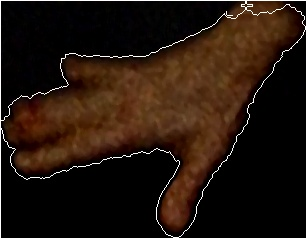
\includegraphics[width=0.25\textwidth]{13sub.jpg}}
    \subfloat[Thresholded]{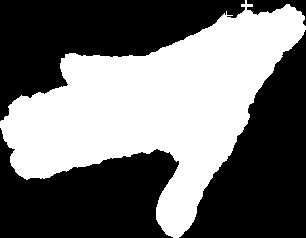
\includegraphics[width=0.25\textwidth]{13bw.jpg}}\\
    \subfloat[Original]{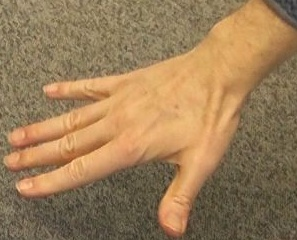
\includegraphics[width=0.25\textwidth]{18orig.jpg}}
    \subfloat[Subtracted]{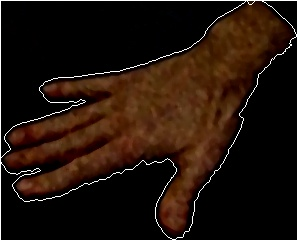
\includegraphics[width=0.25\textwidth]{18sub.jpg}}
    \subfloat[Thresholded]{
\includegraphics[width=0.25\textwidth]{18bw.jpg}}\\
    \subfloat[Original]{
\includegraphics[width=0.25\textwidth]{115orig.jpg}}
    \subfloat[Subtracted]{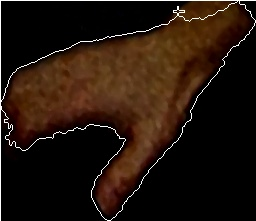
\includegraphics[width=0.25\textwidth]{115sub.jpg}}
    \subfloat[Thresholded]{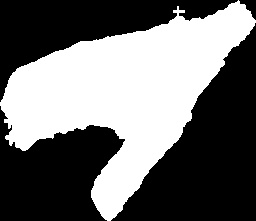
\includegraphics[width=0.25\textwidth]{115bw.jpg}}\\
    \subfloat[Motion History Image]{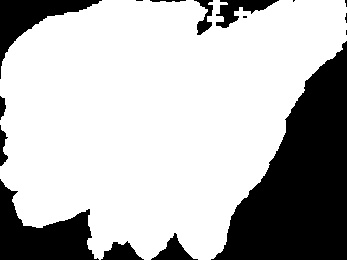
\includegraphics[width=0.25\textwidth]{1mhi.jpg}}
\end{center}
\caption{Images for paper action}
\label{fig:paperSeq}
\end{figure}

\begin{figure}[htp]
\begin{center}
    \subfloat[Original]{
\includegraphics[width=0.25\textwidth]{43orig.jpg}}
    \subfloat[Subtracted]{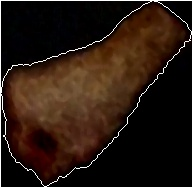
\includegraphics[width=0.25\textwidth]{43sub.jpg}}
    \subfloat[Thresholded]{
\includegraphics[width=0.25\textwidth]{43bw.jpg}}\\
    \subfloat[Original]{
\includegraphics[width=0.25\textwidth]{64orig.jpg}}
    \subfloat[Subtracted]{
\includegraphics[width=0.25\textwidth]{64sub.jpg}}
    \subfloat[Thresholded]{
\includegraphics[width=0.25\textwidth]{64bw.jpg}}\\
    \subfloat[Original]{
\includegraphics[width=0.25\textwidth]{69orig.jpg}}
    \subfloat[Subtracted]{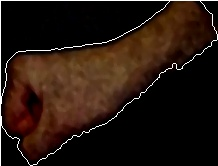
\includegraphics[width=0.25\textwidth]{69sub.jpg}}
    \subfloat[Thresholded]{
\includegraphics[width=0.25\textwidth]{69bw.jpg}}\\
    \subfloat[Motion History Image]{
\includegraphics[width=0.25\textwidth]{6mhi.jpg}}
\end{center}
\caption{Images for rock action}
\label{fig:rockSeq}
\end{figure}

\begin{figure}[htp]
\begin{center}
    \subfloat[Original]{
\includegraphics[width=0.25\textwidth]{82orig.jpg}}
    \subfloat[Subtracted]{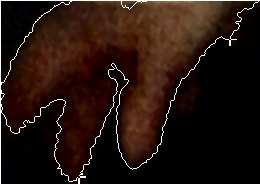
\includegraphics[width=0.25\textwidth]{82sub.jpg}}
    \subfloat[Thresholded]{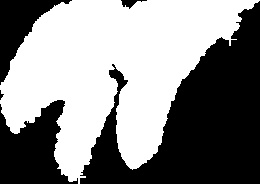
\includegraphics[width=0.25\textwidth]{82bw.jpg}}\\
    \subfloat[Original]{
\includegraphics[width=0.25\textwidth]{89orig.jpg}}
    \subfloat[Subtracted]{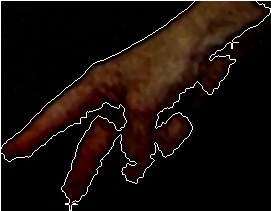
\includegraphics[width=0.25\textwidth]{89sub.jpg}}
    \subfloat[Thresholded]{
\includegraphics[width=0.25\textwidth]{89bw.jpg}}\\
    \subfloat[Original]{
\includegraphics[width=0.25\textwidth]{817orig.jpg}}
    \subfloat[Subtracted]{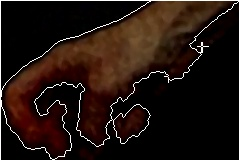
\includegraphics[width=0.25\textwidth]{817sub.jpg}}
    \subfloat[Thresholded]{
\includegraphics[width=0.25\textwidth]{817bw.jpg}}\\
    \subfloat[Motion History Image]{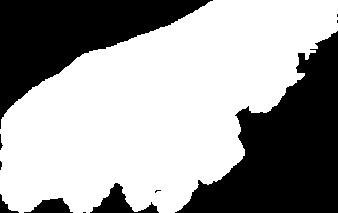
\includegraphics[width=0.25\textwidth]{8mhi.jpg}}
\end{center}
\caption{Images for scissors action}
\label{fig:scissorsSeq}
\end{figure}

\graphicspath{{./}}

\begin{figure}
\begin{center}
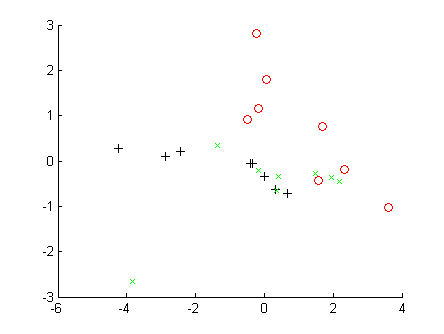
\includegraphics[width=110mm]{paclassplot.png}
\caption{Scatter plot shows dependency between first two principal components used and actual class of an object. Black plus signs indicate "paper" sign , green crosses indicate "rock" sign, red circles indicate "scissors" sign. }
\label{fig:paclassplot}
\end{center}
\end{figure}

Cross validation test results showed that best accuracy over validation data set was achieved by using combination of Hu moments and temporal area of the extracted object as features of the motion image and multi-class SVM for classification. Results for using different feature sets are shown in Table \ref{tab:features}, for using different number of principal components are shown in Table \ref{tab:pca} and for using different classifiers in Table \ref{tab:classify}.

\begin{table}
\begin{center}
\begin{tabular}{| l | r | r |}
\hline
Features & Test set & Validation set \\ \hline
Temporal area of object only & 73.9\% & 54.2\% \\
Hu moments only & 79.3\% & 58.3\% \\
Both & 91.8\% & 87.5\% \\
\hline
\end{tabular}
\end{center}
\caption{Cross validation results when using different sets of features with optimal number of principal components and optimal classifier.}
\label{tab:features}
\end{table}


\begin{table}
\begin{center}
\begin{tabular}{| l | r | r |}
\hline
Number of PC & Test set & Validation set \\ \hline
3 & 87.3\% & 66.7\% \\
4 & 91.8\% & 79.2\% \\
5 & 91.8\% & 87.5\% \\
6 & 95.7\% & 73.3\% \\
7 & 96.0\% & 83.3\% \\
\hline
\end{tabular}
\end{center}
\caption{Cross validation results when using different number of principal components with set of features and optimal classifier.}
\label{tab:pca}
\end{table}

\begin{table}
\begin{center}
\begin{tabular}{| l | r | r |}
\hline
Classifier & Test set & Validation set \\ \hline
Logistic regression & 88.6\% & 66.7\% \\
Multi-class SVM & 91.8\% & 87.5\% \\
\hline
\end{tabular}
\end{center}
\caption{Cross validation results when using different classifiers with optimal set of features and optimal number of principal components.}
\label{tab:classify}
\end{table}
